\documentclass[11pt]{article}
\usepackage[margin=1in]{geometry}
\usepackage{amsmath,amssymb,booktabs,hyperref,listings,xcolor,slashed,enumitem,longtable,graphicx}
\graphicspath{{figs/}}
\hypersetup{colorlinks=true,linkcolor=blue!60!black,urlcolor=blue!60!black}
\lstset{basicstyle=\ttfamily\small,breaklines=true,frame=single,backgroundcolor=\color{gray!6},columns=fullflexible,keepspaces=true}
\newcommand{\ufoamp}{\texttt{ufoamp}}
\newcommand{\mg}{MadGraph5\_aMC@NLO}
\newcommand{\code}[1]{\texttt{#1}}
\newcommand{\M}{\mathcal{M}}

\title{\textbf{\ufoamp}\\[4pt]\large Tree-level amplitudes directly from a UFO model\\[6pt]\normalsize version 1}
\author{Spencer Ellis\\[2pt]\small Brown University}
\date{\today}

\begin{document}
\maketitle
\tableofcontents
\newpage

%=====================================================================
\section{Introduction}
%=====================================================================
\ufoamp{} is a Python library that computes tree-level helicity amplitudes and squared matrix elements directly from a UFO model~\cite{Degrande:2011ua,Darme:2023jdn} --- the same model files \mg{}~\cite{Alwall:2011uj,Alwall:2014hca} uses. You give it a UFO directory, a process such as \code{"u d > u d z z h"}, and a set of four-momenta; it returns
\begin{itemize}[nosep]
\item the helicity amplitudes $\M(h_1,\dots,h_n)$,
\item $|\M|^2$ summed over colours and helicities and averaged over the initial state,
\item polarised pieces of $|\M|^2$ (chosen helicities of external particles, or a polarisation decomposition of the vector bosons exchanged inside the process),
\item all of the above as a function of the model parameters, which can be changed at any time with a function call,
\item and, with the optional JAX backend, derivatives of $|\M|^2$ with respect to parameters and momenta.
\end{itemize}
It is a library, not an event generator. Unlike \mg{}~\cite{Alwall:2014hca}, Sherpa~\cite{Hoche:2014kca} or Whizard/O'Mega~\cite{Moretti:2001zz}, which turn a model and process into generated code, it interprets the model's vertex structures numerically at run time --- in the spirit of ALOHA's contraction of UFO structures with wavefunctions~\cite{deAquino:2011ub}, but without a code-generation step. It operates on events that already exist --- an LHE file, an analysis n-tuple, a set of phase-space points --- and returns quantities a generator does not expose. Typical uses: reweighting a sample to other coupling values, splitting a process into polarisation states, building matrix-element observables, or studying the effect of individual vertices, gauges and width schemes.

\subsection{How it works, in one paragraph}
Nothing about a model is hard-coded. Particles, vertices, coupling expressions and the Lorentz and colour structures of every vertex are read from the UFO and interpreted numerically by a single general routine. Amplitudes are assembled by Berends--Giele recursion~\cite{Berends:1987me} --- off-shell currents built for every subset of external legs and combined through the model's vertices --- so no Feynman diagrams are ever enumerated; this is also the approach of HELAC~\cite{Kanaki:2000ey}, O'Mega~\cite{Moretti:2001zz}, Comix~\cite{Gleisberg:2008fv} and Pepper~\cite{Bothmann:2023gew}. Colour is handled exactly: for processes with gluons the currents carry explicit colour indices (colour-dressed recursion~\cite{Duhr:2006iq}), for quark-line processes the colour sum is done by counting colour loops in the colour-flow basis~\cite{Maltoni:2002mq}, which costs nothing. Events and helicity configurations are processed in batches. Every result is checked against \mg{} on identical phase-space points (\S\ref{sec:validation}).

\subsection{Scope}
Supported: spins 0, 1/2 (Dirac and Majorana, the latter with the fermion-flow rules of ref.~\cite{Denner:1992vza}) and 1; colour singlets, triplets and octets; vertices with any number of legs; Feynman and unitary gauge; fixed-width and complex-mass schemes; any UFO that \mg{} can import, in the original or Python-2 format. Not supported: spin-2 particles, colour sextets, custom propagators and form factors, loop amplitudes.

%=====================================================================
\section{Installation}
%=====================================================================
Requirements: Python $\ge3.10$ and NumPy (installed automatically). Optional: JAX for the compiled and differentiable backend; \mg{} with \code{g++} to run the comparison tools of \S\ref{sec:validation}.
\begin{lstlisting}
pip install ufoamp-1.0.0-py3-none-any.whl        # or:  pip install ufoamp-1.0.0.tar.gz
pip install "ufoamp[jax] @ file:ufoamp-1.0.0.tar.gz"   # with the JAX backend
\end{lstlisting}
This installs the \code{ufoamp} package and the command \code{ufoamp-validate} (the same as \code{python -m ufoamp.validate}). The distribution files are built from the source tree with \code{python -m build}; developers can instead \code{pip install -e /path/to/ufoamp} to work on the source in place. The source tree also carries the test-suite (\code{run\_tests.sh}), the examples and this manual.
Models are UFO directories, for example those under \code{MG5\_aMC/models/}. The test-suite (\S\ref{sec:tests}) uses \mg's Standard Model, found through the environment variable \code{PYAMP\_MG5} (the \mg{} installation) or \code{PYAMP\_SM\_UFO} (the \code{sm} directory).

%=====================================================================
\section{Quick start}
%=====================================================================
\subsection{One event}
\begin{lstlisting}[language=Python]
import numpy as np
from ufoamp.analysis import MatrixElement

# model: any UFO directory; here the Standard Model shipped with MadGraph
me = MatrixElement("/path/to/MG5_aMC/models/sm", "u d > u d h")

# an event: four-vectors [E, px, py, pz] in GeV, in the order of the process string
p = [[500,    0,   0,  500],     # incoming u
     [500,    0,   0, -500],     # incoming d
     [300,  100,  50,  270],     # outgoing u
     [400, -120, -30, -370],     # outgoing d
     [300,   20, -20,  100]]     # outgoing h

print(me.m2(p))                    # |M|^2, colour and spin summed, initial state averaged
print(me.m2_by_helicity(p))        # {(h1, ..., h5): |M|^2} for every helicity configuration

me.set_param({"MH": 200.0})    # change any external parameter of the model ...
print(me.m2(p))                    # ... and evaluate again, no rebuild
\end{lstlisting}
Any external parameter of the UFO can be changed this way: masses, widths, mixing angles, coupling modifiers, Wilson coefficients. Internal parameters and couplings are re-derived from the model's own expressions.

\subsection{An LHE sample}
Samples produced with \mg{} for \code{p p > ...} mix many partonic channels. \code{SampleEvaluator} builds one matrix element per channel the first time it is needed and keeps it:
\begin{lstlisting}[language=Python]
from ufoamp.analysis import SampleEvaluator, read_lhe

ev = SampleEvaluator("/path/to/MG5_aMC/models/sm",
                     param_card="param_card.dat",   # the card of the MadGraph run
                     max_orders={"QCD": 0})         # the sample was generated with QCD=0
events = list(read_lhe("unweighted_events.lhe.gz"))

m2       = ev.m2_sample(events, n_jobs=8)                        # |M|^2 of every event
m2_LLext = ev.m2_sample(events, pol={"z": "L"},  n_jobs=8)       # external Z's longitudinal
m2_LLint = ev.m2_sample(events, vpol="LL",       n_jobs=8)       # internal fusing bosons longitudinal
\end{lstlisting}
Each call returns a NumPy array of $|\M|^2$ values, one per event, in the order of the file. They are squared matrix elements, not weights: a reweighting factor is a ratio of two such arrays (\S\ref{sec:reweighting}), a polarisation fraction is \code{m2\_LLext / m2}. \code{n\_jobs} is the number of processes used in parallel (events are split between them; results are merged in order). The two polarised calls select different things:
\begin{itemize}[nosep]
\item \code{pol=\{"z": "L"\}} restricts the helicities of the \emph{external} $Z$ bosons (those in the process string) to longitudinal --- an exact selection: the LL, LT, TL, TT pieces add up to the total.
\item \code{vpol="LL"} decomposes the propagators of the \emph{internal} vector bosons exchanged between the two quark lines in a vector-boson-fusion process (\S\ref{sec:vpol}) --- a definition rather than an exact selection, meaningful for Higgs production by vector-boson fusion.
\end{itemize}

\subsection{Comparing with \mg}
\begin{lstlisting}
python -m ufoamp.validate --model /path/to/MG5_aMC/models/sm --process "u d > u d h" \
    --orders QCD=0 --mg5 /path/to/MG5_aMC --mg5-model sm
\end{lstlisting}
prints what the model needs and what \ufoamp{} supports, generates the corresponding \mg{} matrix element, and compares the two on random phase-space points (\S\ref{sec:validation}).

%=====================================================================
\section{The \code{MatrixElement} interface}\label{sec:interface}
%=====================================================================
\begin{lstlisting}[language=Python]
MatrixElement(model, process, couplings=None, param_card=None, restrict="default",
              max_orders=None, gauge="auto", scheme="fixed_width", zerowidth_tchannel=False,
              pol_frame="lab", massless_light_quarks=True, drop_vertex=None)
\end{lstlisting}
\begin{description}[nosep]
\item[\code{model}] a UFO directory.
\item[\code{process}] \code{"u d > u d h"} with the particle names of the UFO (\code{w+}, \code{z}, \code{h}, \code{e-}, \code{mu+}, \code{u\textasciitilde}, \dots) or PDG codes.
\item[\code{couplings}] \code{\{parameter: value\}} for any external parameter of the UFO.
\item[\code{param\_card}] an SLHA card, typically the \code{param\_card.dat} of a \mg{} run; \code{DECAY} blocks set widths.
\item[\code{restrict}] a \mg{} restriction card: \code{"default"} applies the model's \code{restrict\_default.dat} if it exists (\mg{} does the same on \code{import model}), a name such as \code{"4FSZeroYukawa"} applies \code{restrict\_<name>.dat}, \code{None} applies nothing. Values in the restriction are overridden by the param card, which is overridden by \code{couplings}.
\item[\code{max\_orders}] coupling-order limits per vertex, e.g.\ \code{\{"QCD": 0\}} for a sample generated with \code{QCD=0}.
\item[\code{gauge}] \code{"auto"}: Feynman gauge if the UFO contains Goldstone bosons, unitary gauge otherwise; or \code{"feynman"} / \code{"unitary"} (\S\ref{sec:gauge}).
\item[\code{scheme}] \code{"fixed\_width"} (real masses in couplings, $iM\Gamma$ in propagators; \mg's choice) or \code{"cms"} (complex masses everywhere).
\item[\code{zerowidth\_tchannel}] set widths to zero in spacelike propagators (\mg's event generation does this by default; its standalone code does not).
\item[\code{pol\_frame}] the frame in which external helicities are defined: \code{"lab"}, \code{"partonic\_cm"} (the frame \mg{} uses for polarised samples), or a list of legs (\S\ref{sec:frames}).
\item[\code{massless\_light\_quarks}] set the $u,d,s,c$ masses and Yukawa couplings to zero, as \mg{} does.
\item[\code{drop\_vertex}] a function \code{(vertex, pdgs) -> bool}; vertices for which it returns \code{True} are removed --- the way to switch off a class of diagrams.
\end{description}
Methods:
\begin{description}[nosep]
\item[\code{m2(momenta, pol=None)}] $|\M|^2$ of one event; \code{pol} restricts external helicities, e.g.\ \code{\{"w+": "L", "w-": "T"\}} or \code{\{4: [1, -1]\}} (leg index, list of helicities).
\item[\code{m2\_events(events, pol=None, n\_jobs=1, chunk=32)}] the same for an array of events.
\item[\code{m2\_by\_helicity(momenta)}] $|\M|^2$ for every helicity configuration, in one pass. External helicities do not interfere, so any polarised quantity is a sum over its keys.
\item[\code{m2\_polarized(momenta, ["z"])}] \code{\{"LL", "LT", "TL", "TT"\}} for the named massive vector bosons; the four add up to the total.
\item[\code{helicity\_amplitudes(momenta)}] the amplitudes $\M$ themselves (for coloured processes, a tensor over the external colour indices).
\item[\code{set\_param(\{...\})}] change parameters. \code{set\_amp\_orders(\{"NP": (0, 1)\})} keeps only the part of the amplitude with total coupling order in the given window (\mg's \code{NP<=1}; see \S\ref{sec:eft}). \code{set\_vpol("LL")} activates the internal decomposition (\S\ref{sec:vpol}).
\item[\code{param(name)}] the value of a parameter after all cards and overrides.
\end{description}
Helicity labels: fermions $\pm1$ (for $\pm\tfrac12$), massive vectors $\pm1,0$, massless vectors $\pm1$, scalars $0$. In \code{pol}, the letters \code{L}, \code{T}, \code{+}, \code{-} stand for $\{0\}$, $\{+1,-1\}$, $\{+1\}$, $\{-1\}$.

\subsection{Conventions}
\begin{itemize}[nosep]
\item Four-vectors are $(E,p_x,p_y,p_z)$ in GeV with metric $(+,-,-,-)$; helicity spinors and polarisation vectors follow the HELAS conventions~\cite{Murayama:1992gi,Hagiwara:1985yu}; events are listed initial particles first, then final, in the order of the process string.
\item $|\M|^2$ is summed over final helicities and colours and averaged over initial helicities and colours. It is the bare squared amplitude: the factor $1/n!$ for $n$ identical particles in the final state is \emph{not} included. That factor belongs to the phase-space integration --- it prevents counting the same final state $n!$ times --- and \mg's standalone code folds it into its matrix element because a cross section is what it is built for. \ufoamp{} leaves it out so that per-event quantities (helicity fractions, reweighting ratios, observables) are unaffected; when comparing a single number with \mg, multiply \ufoamp's value by $1/n!$.
\item Widths are kept in all propagators, spacelike ones included, unless \code{zerowidth\_tchannel=True}.
\item Light-quark masses and Yukawa couplings are zero by default.
\end{itemize}

%=====================================================================
\section{Polarisation}
%=====================================================================
\subsection{External particles}
The helicities of the external particles are chosen with \code{pol} or read off \code{m2\_by\_helicity}. Because $|\M|^2$ summed over the helicities of a particle is a sum of the squares of its helicity amplitudes, the pieces are exact and additive: \code{m2\_polarized} for two $Z$ bosons returns LL, LT, TL and TT which add up to the total. This is the quantity \mg{} generates when a process is written as \code{z\{0\} z\{0\}} (longitudinal) or \code{z\{T\} z\{T\}} (transverse)~\cite{BuarqueFranzosi:2019boy}, provided the same frame is used (\S\ref{sec:frames}); validation study~3 shows the two agree.

\subsection{Frames}\label{sec:frames}
The helicity of a massive particle depends on the frame in which it is measured. \ufoamp{} uses the momenta as you pass them (\code{pol\_frame="lab"}); \code{pol\_frame="partonic\_cm"} first boosts every event to the rest frame of the two incoming partons, which is the frame \mg{} uses for its polarised samples; a list of leg indices selects the rest frame of their summed momentum. The helicity-summed $|\M|^2$ does not depend on the choice (it is a Lorentz scalar); the polarised pieces do, by up to $\sim15\%$ on typical vector-boson-fusion events.

\subsection{Internal vector bosons: the propagator decomposition}\label{sec:vpol}
In vector-boson fusion, $q\,q\to q\,q + X$ with $X$ produced by the fusion of two vector bosons, the bosons whose polarisation one would like to know are internal and off shell, so their ``polarisation'' needs a definition. \ufoamp{} implements the propagator decomposition of Ballestrero, Maina and Pelliccioli~\cite{Ballestrero:2017bxn,Ballestrero:2019qoy} (the on-shell-projection alternative of ref.~\cite{Denner:2020bcz} is not implemented): for each vector boson radiated off a quark line, the numerator of its propagator is written as a sum over polarisation vectors,
\[
-g^{\mu\nu}+\frac{k^\mu k^\nu}{M^2}=\underbrace{\sum_{\lambda=\pm}\epsilon_\lambda^\mu\epsilon_\lambda^{\nu*}}_{T}\;+\;\underbrace{\mathrm{sgn}(k^2)\,\epsilon_L^\mu\epsilon_L^{\nu*}}_{L}\;+\;\underbrace{k^\mu k^\nu\Big(\frac{1}{M^2}-\frac{1}{k^2}\Big)}_{S},
\]
with the vectors built from the off-shell momentum $k$ in a chosen frame (by default the rest frame of $X$), and only the selected terms are kept: \code{set\_vpol("LL")} keeps $L$ for both bosons, \code{"TT"} keeps $T$ for both, \code{"A"} keeps everything and reproduces the full result. Two properties to keep in mind:
\begin{itemize}[nosep]
\item The pieces \emph{interfere}: $|\M_{LL}|^2+|\M_{LT}|^2+|\M_{TL}|^2+|\M_{TT}|^2\neq|\M|^2$. This is an amplitude-level definition, not a partition of the cross section; the interference terms are physical and must be kept~\cite{Ballestrero:2019qoy}.
\item It is meaningful only when every diagram of the process contains the two fused bosons, as in Higgs production by vector-boson fusion ($q q\to q q h$, $q q\to q q h h$). In processes where the vector bosons also radiate directly off the quark lines (e.g.\ $q q\to q q z z$), the diagrams that are not decomposed dominate every selection and the pieces carry no polarisation information; use the external-particle helicities of the $Z$'s instead.
\end{itemize}

%=====================================================================
\section{Changing couplings: reweighting and morphing}\label{sec:reweighting}
%=====================================================================
Because parameters are run-time arguments, the ratio of $|\M|^2$ at two parameter points is available for every event:
\begin{lstlisting}[language=Python]
ev.set_param({"MH": 125.0});  m2_sm  = ev.m2_sample(events)
ev.set_param({"MH": 200.0});  m2_new = ev.m2_sample(events)
w = m2_new / m2_sm          # multiply into the event weights of the sample
\end{lstlisting}
An event sample generated at one parameter point, weighted by $w$, is distributed as a sample generated at the new point: parton densities, flux and phase-space density are the same for both and cancel in the ratio. This is matrix-element reweighting as automated in \mg{}~\cite{Artoisenet:2010cn,Mattelaer:2016gcx}. The only limitation is statistical: if the new point enhances a region the original sample barely populates, a few events carry large weights. The effective sample size $(\sum w)^2/\sum w^2$ per bin measures this and should be checked.

\paragraph{Morphing.} The polynomial structure used here is the morphing technique of refs.~\cite{ATL-PHYS-PUB-2015-047,Brehmer:2019xox}. When the amplitude is linear in the parameters --- coupling modifiers $\kappa$, or an effective field theory with one operator insertion per amplitude --- $|\M|^2$ is a quadratic polynomial in them: for $\M=A+c_1B+c_2C$,
\[
|\M|^2=p_0+p_1c_1+p_2c_2+p_3c_1^2+p_4c_2^2+p_5c_1c_2 .
\]
The six coefficients of an event are determined exactly from six evaluations at six parameter points (solving a $6\times6$ linear system); stored per event, they give the weight for any $(c_1,c_2)$ without further matrix-element calls, the interference term $p_1c_1+p_2c_2$ on its own, and the observables $p_1/p_0$, $p_2/p_0$ that are optimal for measuring $c_1$, $c_2$~\cite{Atwood:1991ka,Diehl:1993br,Brehmer:2016nyr}. A seventh evaluation at a test point confirms the polynomial form. The same holds per helicity class using \code{m2\_by\_helicity}.

\subsection{Effective field theories}\label{sec:eft}
UFOs for effective field theories carry a coupling order (\code{NP} in SMEFTsim~\cite{Brivio:2017btx,Brivio:2020onw}) counting operator insertions. With every insertion kept, $|\M|^2$ is a polynomial of higher degree (diagrams with two insertions, and parameters entering through input-scheme relations); \code{set\_amp\_orders(\{"NP": (0, 1)\})} keeps only the part of the amplitude with at most one insertion, reproducing \mg's \code{NP<=1} and making $|\M|^2$ exactly quadratic. \code{(1, 1)} keeps the single-insertion part alone, so that $|\M_{0+1}|^2-|\M_0|^2-|\M_1|^2$ is the pure interference between the Standard Model and the operator.

%=====================================================================
\section{Gauge and widths}\label{sec:gauge}
%=====================================================================
Massive vector bosons can be treated in Feynman gauge (propagator $-ig^{\mu\nu}/D$, with Goldstone bosons as internal particles) or in unitary gauge ($-i(g^{\mu\nu}-k^\mu k^\nu/M^2)/D$, no Goldstones); a UFO supports Feynman gauge only if it contains Goldstone bosons, which \ufoamp{} detects. The two give identical results for a physical process --- validation study~2 shows this to $10^{-13}$ for $W^+W^-\to hh$ --- with one exception: when unstable particles carry a width, propagators inside larger sub-amplitudes break the identity by terms of order $\Gamma/M$ (the naive width spoils the cancellation between the $k^\mu k^\nu$ term and the Goldstone exchange, a well-known effect~\cite{Baur:1995aa}). With widths set to zero the gauges always agree exactly. \mg's standalone code is unitary gauge with widths kept in every propagator; \code{gauge="unitary"} reproduces it.

The complex-mass scheme~\cite{Denner:1999gp,Denner:2005fg} (\code{scheme="cms"}) uses $M^2\to M^2-iM\Gamma$ in the couplings as well as in the propagators and restores gauge independence when all external particles are stable. For processes with external unstable bosons on their real mass shell (e.g.\ $q q\to q q z z$) a difference of order $\Gamma/M$ between gauges remains in every scheme; it is a property of tree-level calculations with widths, not of \ufoamp.

%=====================================================================
\section{The JAX backend}\label{sec:jax}
%=====================================================================
\begin{lstlisting}[language=Python]
from ufoamp.jaxme import JaxMatrixElement
jme = JaxMatrixElement(me, params=["MH"])   # me: a MatrixElement; params: parameters to differentiate
jme.m2(events)                              # |M|^2, compiled; identical to me.m2_events
jme.grad_params(events)                     # d|M|^2/dMH per event
jme.hessian_params(events)                  # second derivatives
jme.grad_momenta(events)                    # d|M|^2/dp^mu per event and leg
\end{lstlisting}
The chain parameters $\to$ couplings $\to$ amplitude $\to$ $|\M|^2$ is traced once per process and compiled by XLA~\cite{Bradbury:2018jax}. Differentiable matrix elements were first provided for \mg{} processes by MadJax~\cite{Heinrich:2022xfa}, which generates JAX code per process; here the generic evaluator is traced instead; the Python bookkeeping of the recursion then runs only at compile time. Results equal the NumPy backend to machine precision. The derivatives come from automatic differentiation, so they are exact rather than finite differences (validation study~6 checks them against the exact derivatives of the morphing polynomial). This is what makes the backend useful beyond speed: $\partial|\M|^2/\partial c$ per event, divided by $|\M|^2$, is the matrix-element observable that is optimal for measuring the parameter $c$~\cite{Atwood:1991ka,Diehl:1993br} (\S\ref{sec:reweighting}); the same derivatives give the interference term of an effective-field-theory operator per event and per helicity class, and second derivatives give the sensitivity (Fisher information) of a measurement~\cite{Brehmer:2016nyr}. One restriction: parameters that enter particle masses or widths (which are used as plain numbers in the wavefunctions and propagators) cannot be differentiated; coupling modifiers, Wilson coefficients and couplings such as $\alpha_s$ can. On a CPU the compiled matrix element is several times faster than the NumPy path for processes with up to six external particles (0.2 versus 1.5\,ms per event for $ud\to udhh$); processes with many helicity configurations are better served by a GPU. Its main value is the derivatives. Requires \code{pip install jax jaxlib}.

%=====================================================================
\section{Comparing with \mg{} and the test-suite}\label{sec:validation}
%=====================================================================
\subsection{The comparison tool}
\code{ufoamp.mg5ref.MG5Reference(mg5\_dir, model, process)} asks \mg{} to generate its own C++ matrix element for the process (``standalone'' mode, which needs only \code{g++}), compiles it, and evaluates it on any momenta from Python with the same parameter card. \code{ref.compare(me, events)} reports the largest relative difference between \ufoamp{} and \mg{} on those events, taking care of the $1/n!$ factor. The two codes share nothing --- \mg{} enumerates Feynman diagrams and uses helicity routines generated by ALOHA~\cite{deAquino:2011ub} and its own colour treatment --- so agreement at $10^{-14}$ is a strong statement, and a disagreement points at a convention that must be matched: the model's restriction card, the coupling orders, the gauge, the widths in $t$-channel propagators, the $1/n!$ factor. \code{python -m ufoamp.validate} wraps this for any model and process and can store the reference values in a file so the comparison can be repeated without \mg.

\subsection{The test-suite}\label{sec:tests}
\code{./run\_tests.sh} runs a fixed set of checks on \mg's Standard Model, each of which must print \code{PASS}: comparisons with textbook formulas ($e^+e^-\to\mu^+\mu^-$ with and without the $Z$, Bhabha scattering, $\sigma=4\pi\alpha^2/3s$, the seven massless QCD $2\to2$ processes of ref.~\cite{Ellis:1996mzs}), the longitudinal gauge cancellation in $e^+e^-\to W^+W^-$, Feynman versus unitary gauge, independence of the result from the order in which the external particles are listed (the consistency check \mg{} itself performs on new models~\cite{Alwall:2011uj}), the coupling-order limits and helicity frames, the JAX backend against NumPy and its derivatives against an exact result, and \mg{} standalone on eight processes. It needs only \code{PYAMP\_MG5} (or \code{PYAMP\_SM\_UFO}); the \mg{} comparison is skipped when \mg{} or \code{g++} is absent.

%=====================================================================
\section{Validation studies}\label{sec:studies}
%=====================================================================
The six studies below were run against \mg{}~3.5.16 with three UFO models placed in its \code{models/} directory: the Standard Model shipped with \mg{} (\code{sm}); the HHVBF model of vector-boson-fusion Higgs-pair production with coupling modifiers $C_V$, $C_{2V}$, $C_3$; and SMEFTsim~3~\cite{Brivio:2020onw} (U35, $M_W$ input scheme) for the effective-field-theory checks. Random phase-space points are generated with RAMBO~\cite{Kleiss:1985gy}. Each study tests one capability against an exact expectation or against \mg. All checks passed at tolerances fixed before running; every number quoted is in the studies' result files.

\subsection{Study 1: $e^+e^-\to W^+W^-$ --- helicity decomposition and the gauge cancellation}
\textbf{What is tested.} That \ufoamp{} splits $|\M|^2$ correctly by the helicities of the $W$ bosons, and that its treatment of the three diagrams of this process (photon exchange, $Z$ exchange, neutrino exchange) has the correct relative signs.

\textbf{Figure~\ref{fig:s1a}} shows $|\M|^2$ against the scattering angle at three collision energies, split into $W$ pairs that are both longitudinal (LL), both transverse (TT) or mixed. The three curves add up to the total exactly (to $4\times10^{-16}$), and the fraction of each class integrated over the angle agrees with three separate \mg{} cross-section calculations for \code{w+\{0\}w-\{0\}}, \code{w+\{T\}w-\{T\}} and unpolarised pairs within their statistical errors (pulls below $0.4\sigma$). The longitudinal fraction falls from 8\% at 200\,GeV to 1\% at 1\,TeV, as it should.

\textbf{Figure~\ref{fig:s1b}} is the classic test of the electroweak theory: each of the three diagrams on its own gives a longitudinal amplitude squared that grows like $s^2$ --- the top panel shows the three growing curves, and the bottom panel shows their ratio between successive doublings of the energy approaching 16 ($=2^4$). Their sum is the flat curve in the top panel, whose doubling ratio approaches 1: the growing pieces cancel to one part in $10^7$ at 5\,TeV. This cancellation happens only if every sign and momentum convention in the three diagrams is right, and it demonstrates that \ufoamp{} lets you switch individual diagram classes on and off (with \code{drop\_vertex}).

\textbf{\mg.} On ten random points at 500\,GeV, \ufoamp{} agrees with \mg{} to $1.5\times10^{-14}$ for the unpolarised $|\M|^2$ and to $6.9\times10^{-14}$ for the longitudinal piece against \mg's \code{w+\{0\}w-\{0\}}.
\begin{figure}[htbp]\centering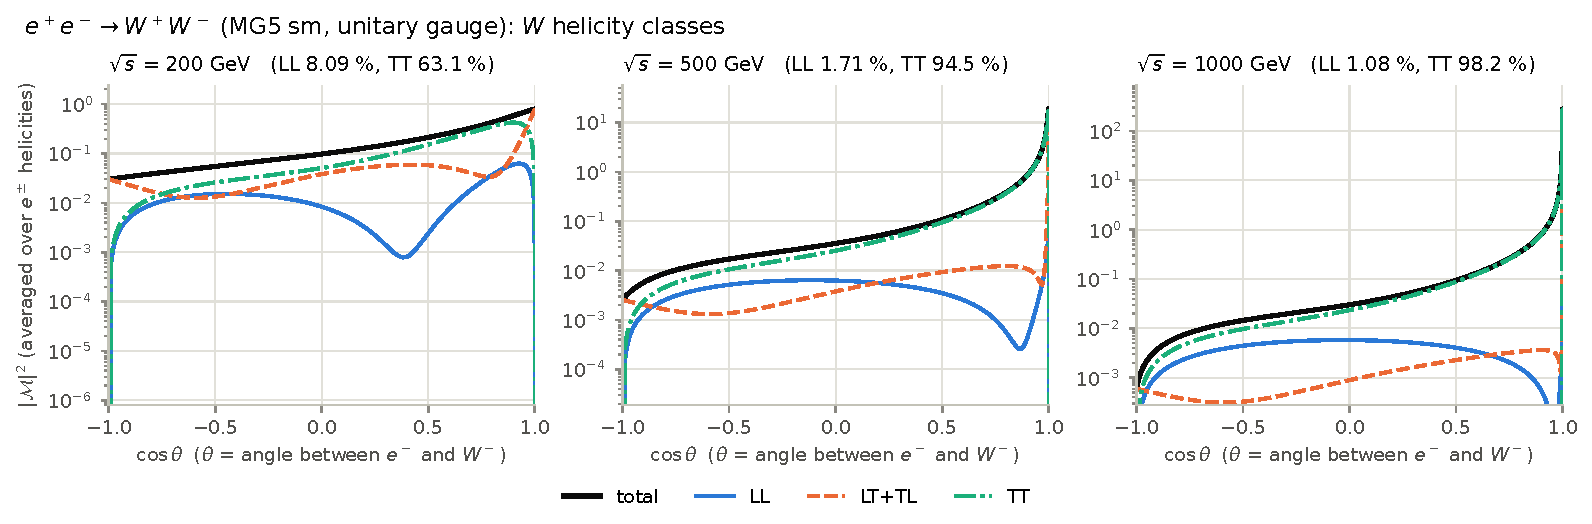
\includegraphics[width=0.9\textwidth]{study1_fig_1a.pdf}\caption{Study 1: $|\M|^2$ for $e^+e^-\to W^+W^-$ versus the scattering angle, split by the helicities of the two $W$ bosons, at three energies.}\label{fig:s1a}\end{figure}
\begin{figure}[htbp]\centering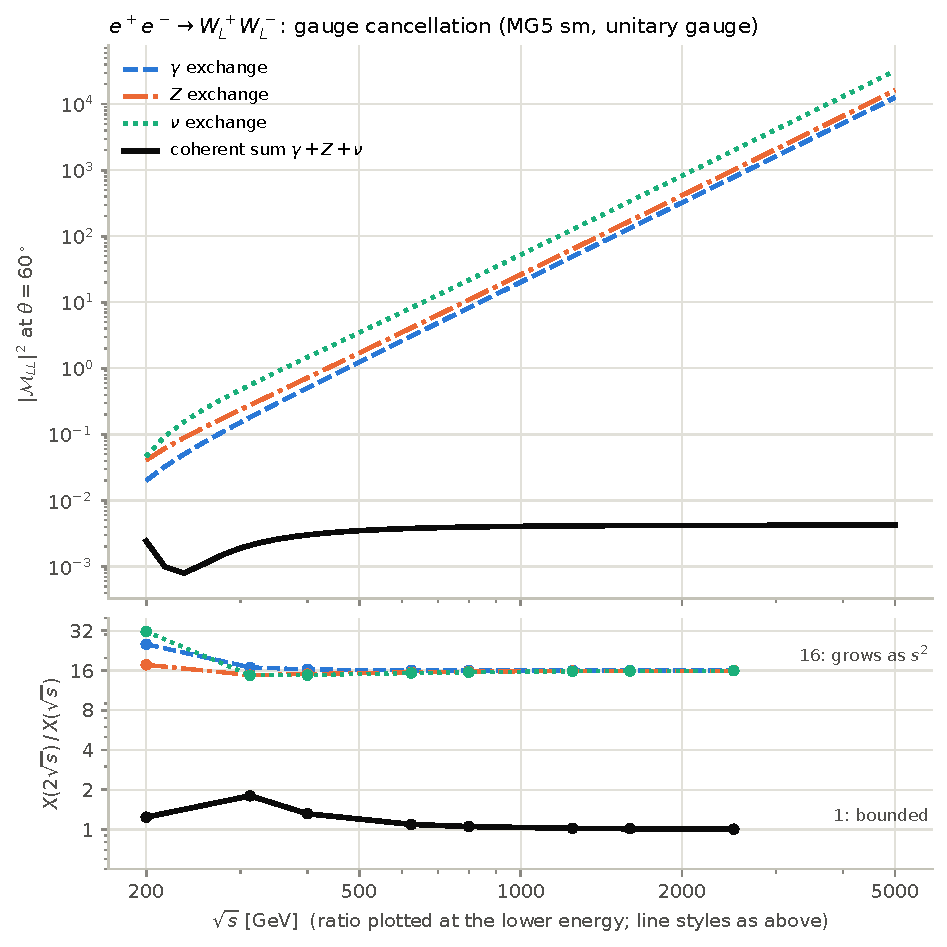
\includegraphics[width=0.75\textwidth]{study1_fig_1b.pdf}\caption{Study 1: the longitudinal gauge cancellation. Top: $|\M_{LL}|^2$ from each exchanged particle and from their coherent sum, versus energy. Bottom: ratio between successive doublings of the energy --- 16 for a term growing like $s^2$, 1 for a constant.}\label{fig:s1b}\end{figure}

\subsection{Study 2: $W^+W^-\to hh$ --- Goldstone equivalence and gauge independence}
\textbf{What is tested.} Two textbook properties: at high energy the amplitude for longitudinal $W$ bosons equals the amplitude for the Goldstone bosons they ``eat'' (the equivalence theorem~\cite{Cornwall:1974km,Lee:1977eg,Chanowitz:1985hj}), and the result does not depend on the gauge.

\textbf{Figure~\ref{fig:s2a}} shows the ratio $r$ of the two amplitudes, $|\M(W_LW_L\to hh)|/|\M(G^+G^-\to hh)|$, versus energy. \ufoamp{} computes both directly, the second with the Goldstone bosons as external particles in Feynman gauge. With widths switched off (blue), $r$ approaches 1 exactly as the theorem predicts, with a correction proportional to $M_W^2/s$: the quantity $(r-1)\,s/M_W^2$ is constant to 0.5\% between 4 and 8\,TeV. With the $W$ width kept in the exchanged $W$ (orange), $r$ settles at a small distance from 1 proportional to $\Gamma_W/M_W$ (with a coefficient 0.558, constant to 0.07\%) --- a known property of putting a width into a propagator by hand, which spoils the identity behind the theorem by a term of that size. The plot therefore shows both that the theorem holds in \ufoamp{} and how large the width effect is.

\textbf{Gauge independence.} The nine helicity amplitudes of $W^+W^-\to hh$ computed in Feynman gauge (with Goldstone exchange) and in unitary gauge (without) agree to $1.5\times10^{-13}$ at 1 and 2\,TeV, with and without widths. \textbf{\mg}: $1.0\times10^{-14}$ on five points.
\begin{figure}[htbp]\centering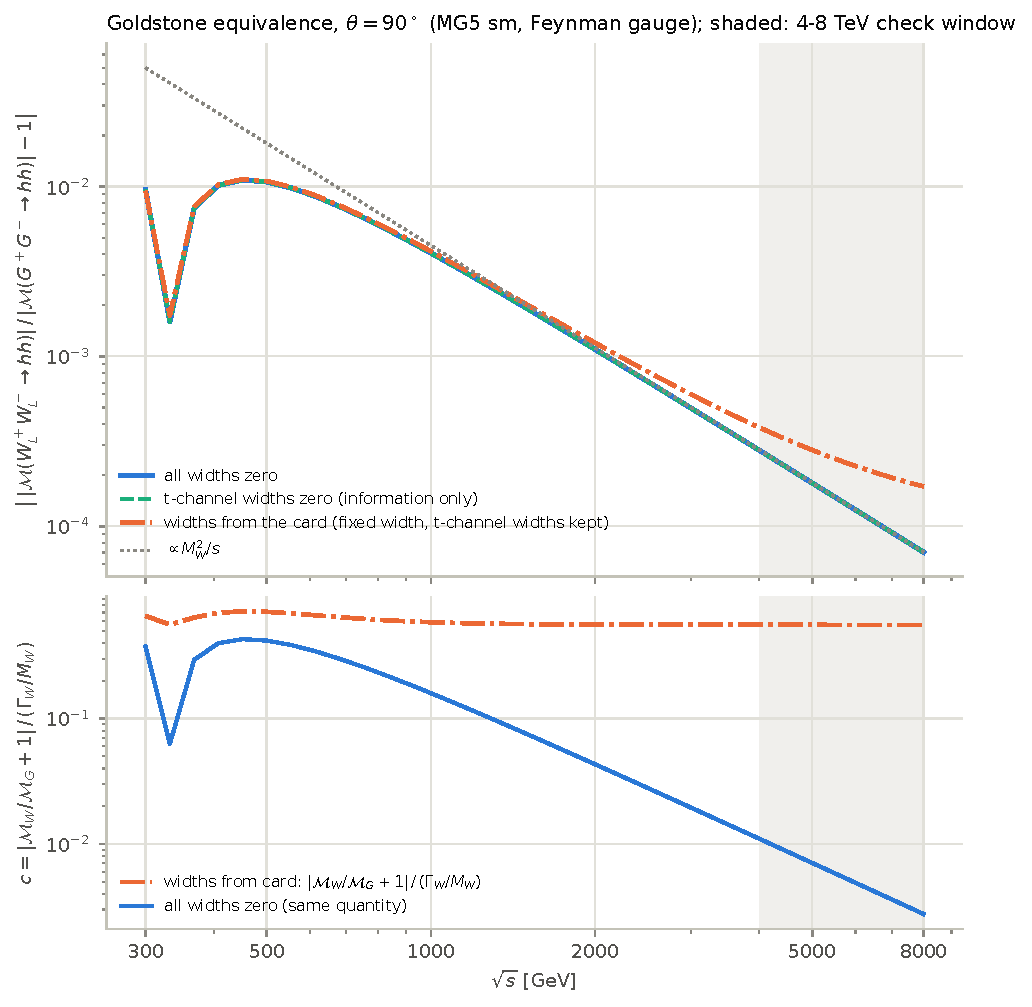
\includegraphics[width=0.8\textwidth]{study2_fig_2a.pdf}\caption{Study 2: ratio of the longitudinal $W$ amplitude to the Goldstone amplitude for $W^+W^-\to hh$ versus energy, for three treatments of the $W$ width.}\label{fig:s2a}\end{figure}

\subsection{Study 3: $pp\to zzjj$ --- polarisation of the $Z$ bosons}
\textbf{What is tested.} That the helicity selection of external particles gives the same physics as \mg's polarised event generation, on a realistic $2\to4$ process with 50\,000 events.

\textbf{Figure~\ref{fig:s3a}} shows, event by event on a \mg{} sample of $pp\to zzjj$ (electroweak production), the fraction of $|\M|^2$ in which both $Z$'s are longitudinal (LL), both transverse (TT) or mixed, as a function of the $ZZ$ invariant mass, defined once in the laboratory frame and once in the partonic centre-of-mass frame. The two definitions differ at low mass and converge at high mass, illustrating that the helicity of a massive particle is frame dependent; the total $|\M|^2$ is the same in both frames for every one of the 50\,000 events (to better than $10^{-10}$), as it must be.

\textbf{Figure~\ref{fig:s3b}} is the decisive test. \mg{} can generate samples with the $Z$'s forced to be longitudinal (\code{z\{0\}z\{0\}}) or transverse (\code{z\{T\}z\{T\}})~\cite{BuarqueFranzosi:2019boy}. Weighting each event of the unpolarised sample by \ufoamp's ratio $|\M_{LL}|^2/|\M|^2$ (in the partonic frame, the one \mg{} uses) must reproduce the longitudinal sample; the figure compares the two in four distributions --- the $ZZ$ mass, the transverse momentum of a $Z$, the decay angle $|\cos\theta^*|$ and the azimuthal angle between the jets --- and likewise for TT. All eight comparisons agree statistically ($p$-values above 0.065), and the total rates agree within one standard deviation. This establishes that \ufoamp's external-helicity selection is the same quantity as \mg's polarised generation.

\textbf{\mg.} On 20 events of each of the three most populated partonic channels, $|\M|^2$ agrees to $9.9\times10^{-14}$.
\begin{figure}[htbp]\centering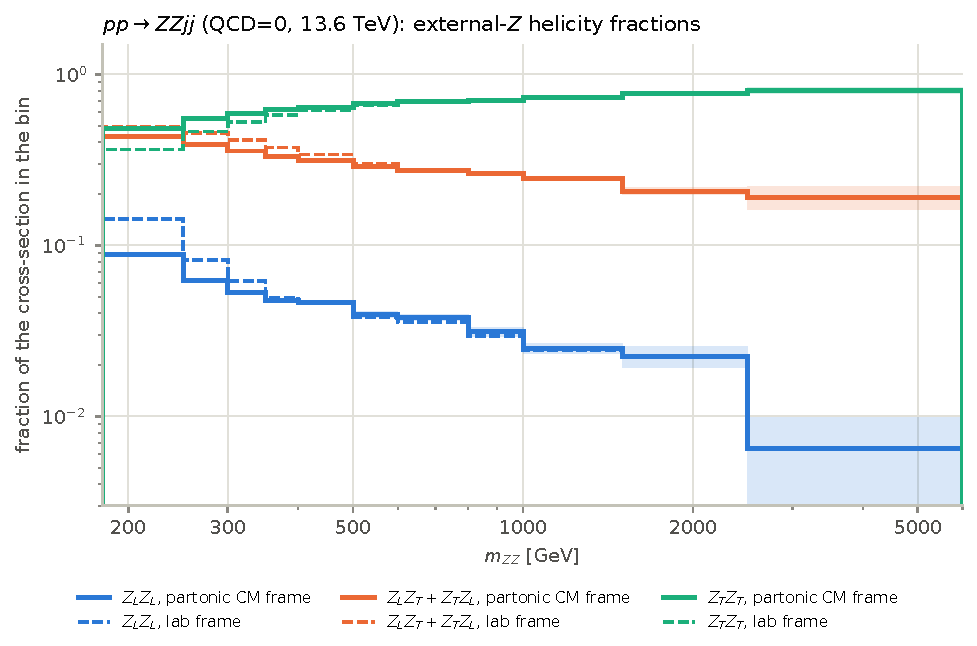
\includegraphics[width=0.9\textwidth]{study3_fig_3a.pdf}\caption{Study 3: fractions of $|\M|^2$ by the helicities of the two $Z$ bosons versus $m_{ZZ}$, in the laboratory and in the partonic centre-of-mass frame.}\label{fig:s3a}\end{figure}
\begin{figure}[htbp]\centering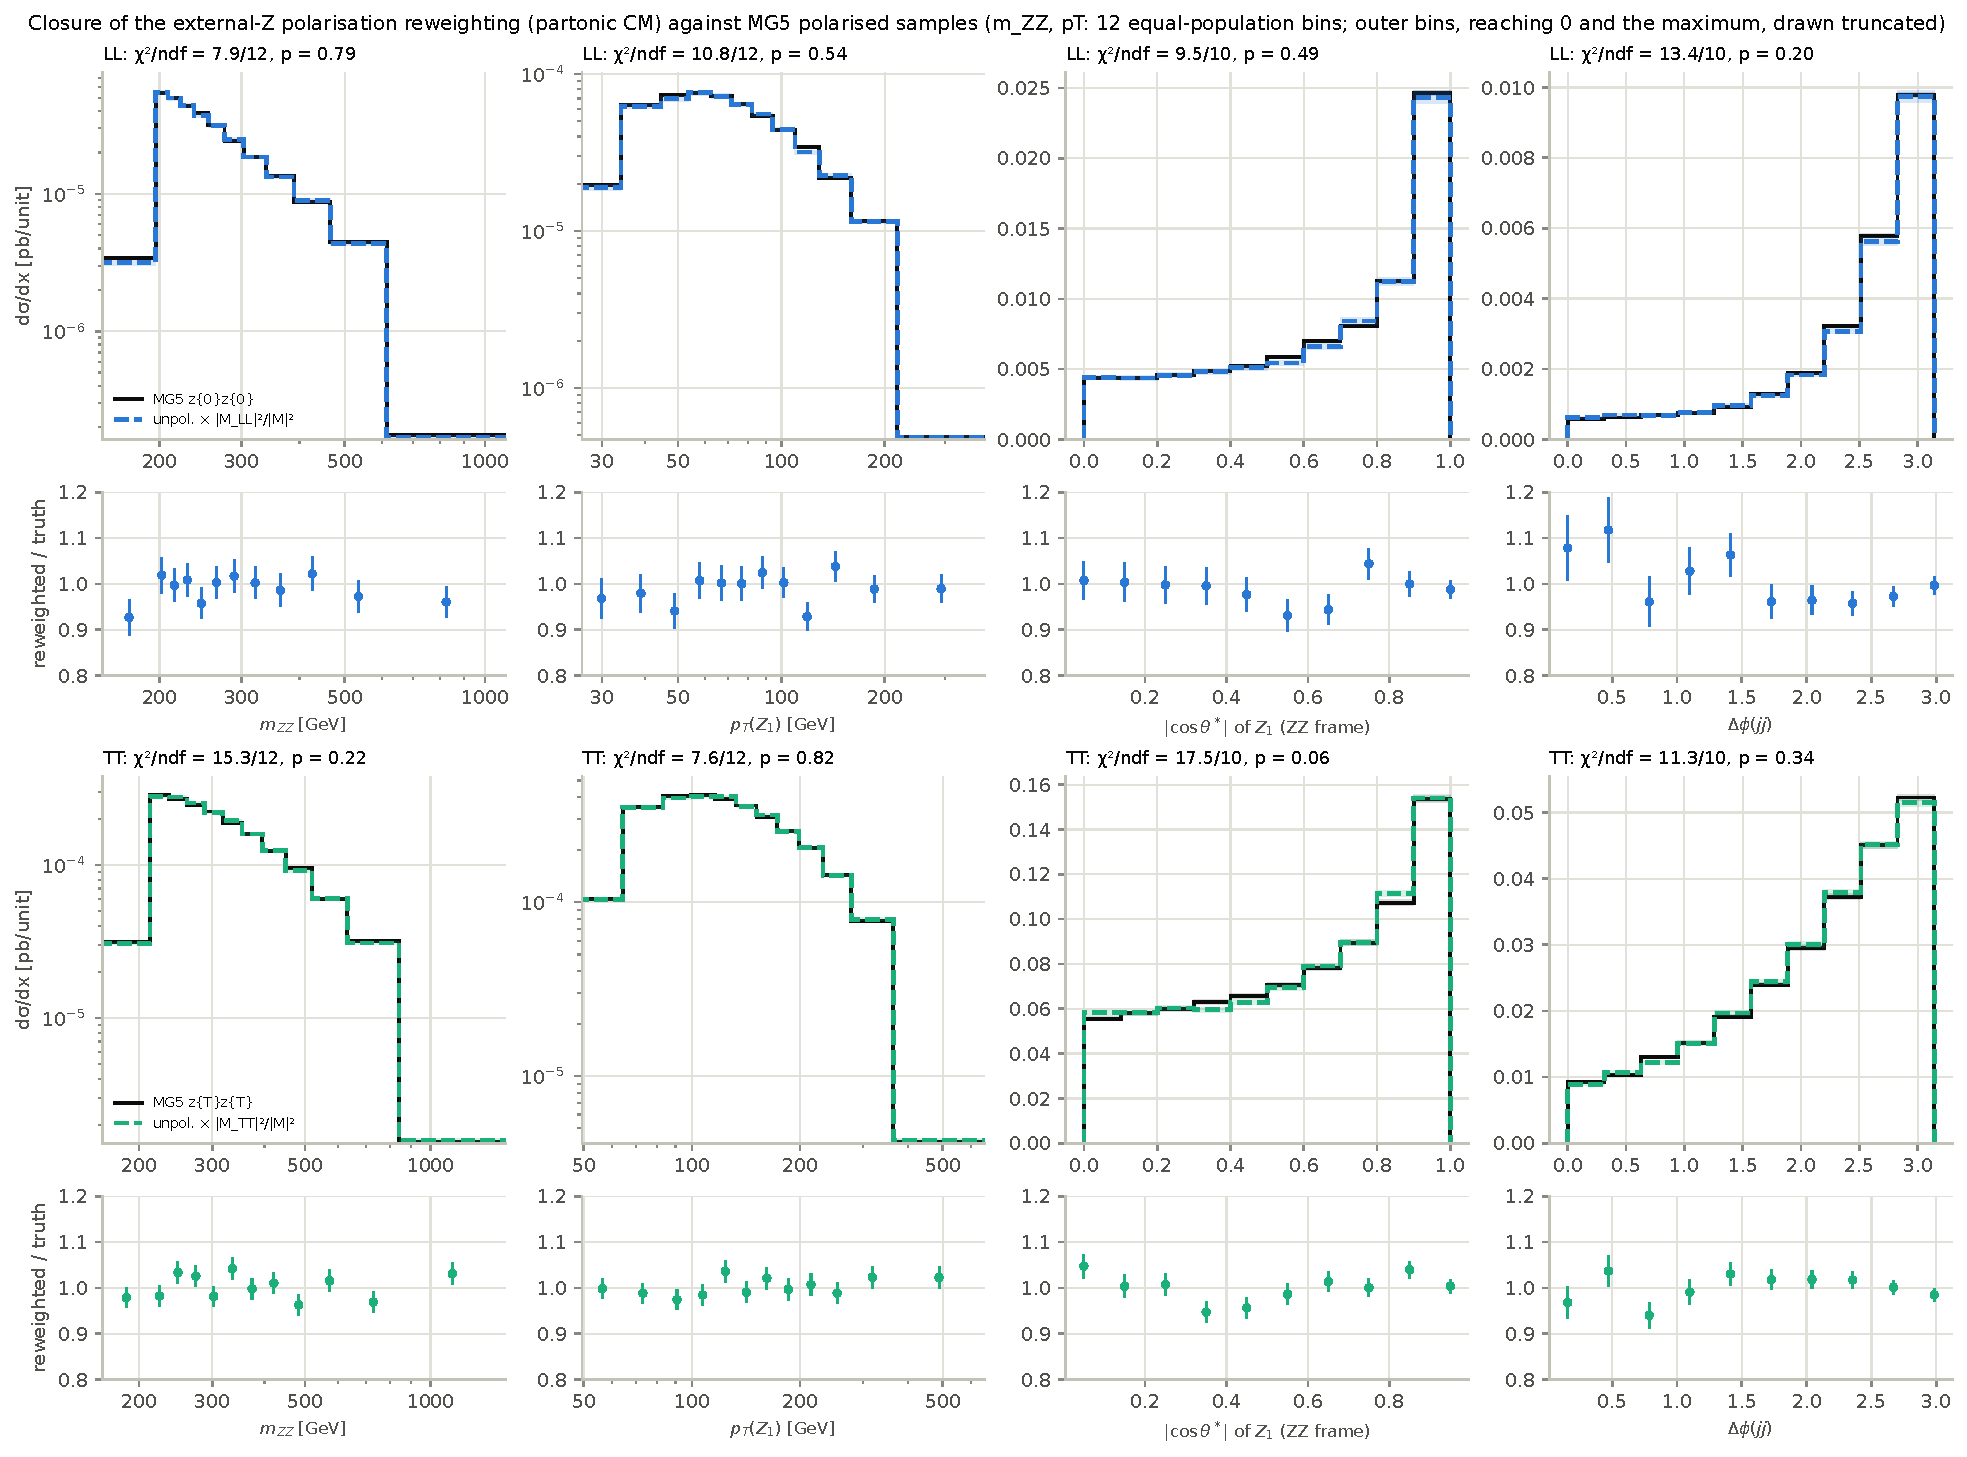
\includegraphics[width=0.9\textwidth]{study3_fig_3b.pdf}\caption{Study 3: the unpolarised \mg{} sample weighted by \ufoamp's LL (resp.\ TT) fraction, compared with \mg's samples generated with longitudinal (resp.\ transverse) $Z$'s.}\label{fig:s3b}\end{figure}

\subsection{Study 4: $pp\to hhjj$ --- coupling modifiers and reweighting}
\textbf{What is tested.} That changing coupling values at run time does what it should: the dependence of $|\M|^2$ on the Higgs coupling modifiers $C_{2V}$ (the $VVhh$ vertex) and $C_3$ (the $hhh$ vertex) has the form the theory dictates, and reweighting a sample with \ufoamp{} agrees with \mg's own reweighting.

\textbf{Figure~\ref{fig:s4a}.} With $C_V=1$ the amplitude is $A+C_{2V}B+C_3C$, so $|\M|^2$ must be a quadratic polynomial in $(C_{2V},C_3)$ with six coefficients. \ufoamp{} determines the six coefficients of every event from six evaluations and then predicts $|\M|^2$ at five other coupling points; the figure shows the difference between prediction and direct evaluation for all 50\,000 events --- below $10^{-11}$ everywhere. The coefficients are the same whichever six points are used (to $2\times10^{-13}$). This is the basis of morphing (\S\ref{sec:reweighting}): once stored, they give the weight for any coupling point without further computation.

\textbf{Reweighting.} \mg{} has its own reweighting module~\cite{Mattelaer:2016gcx}, which recomputes each event's weight at new coupling values. Running it on the same sample to $(C_V,C_{2V},C_3)=(1,1.2,1.5)$ and $(1,2,1)$ and comparing its weight ratio with \ufoamp's, event by event, gives agreement at the level of the eight significant digits with which \mg{} writes its weights (median difference $6\times10^{-9}$, 99.9\% of events below $7\times10^{-8}$). The few events where the two differ more were recomputed with \mg's standalone matrix element, which agrees with \ufoamp{} to $1.5\times10^{-12}$: on those events it is \mg's reweighting module that departs from \mg's own matrix element.

\textbf{Figure~\ref{fig:s4c}} illustrates a property of the HHVBF model itself that \ufoamp{} makes visible. The model multiplies only the physical Higgs vertices by $C_V$, $C_{2V}$, $C_3$ and leaves the Goldstone-boson vertices unchanged, so away from the Standard-Model point it is not gauge invariant (the $\kappa$ framework is defined for rates, not amplitudes~\cite{Heinemeyer:2013tqa}). The figure shows the coefficient of the energy growth of the longitudinal $W_LW_L\to hh$ amplitude for four choices of $(C_V,C_{2V})$: in Feynman gauge it is $|C_{2V}-1|$, in unitary gauge $|C_{2V}-C_V^2|$ (both to $7\times10^{-4}$). The two coincide only for $C_V=1$. Practically: $C_{2V}$ and $C_3$ can be varied freely; varying $C_V$ gives gauge-dependent results with this model.

\textbf{\mg.} $|\M|^2$ agrees to $5.6\times10^{-13}$ on sample events of the seven most populated channels, at the Standard-Model point and at the two other coupling points.
\begin{figure}[htbp]\centering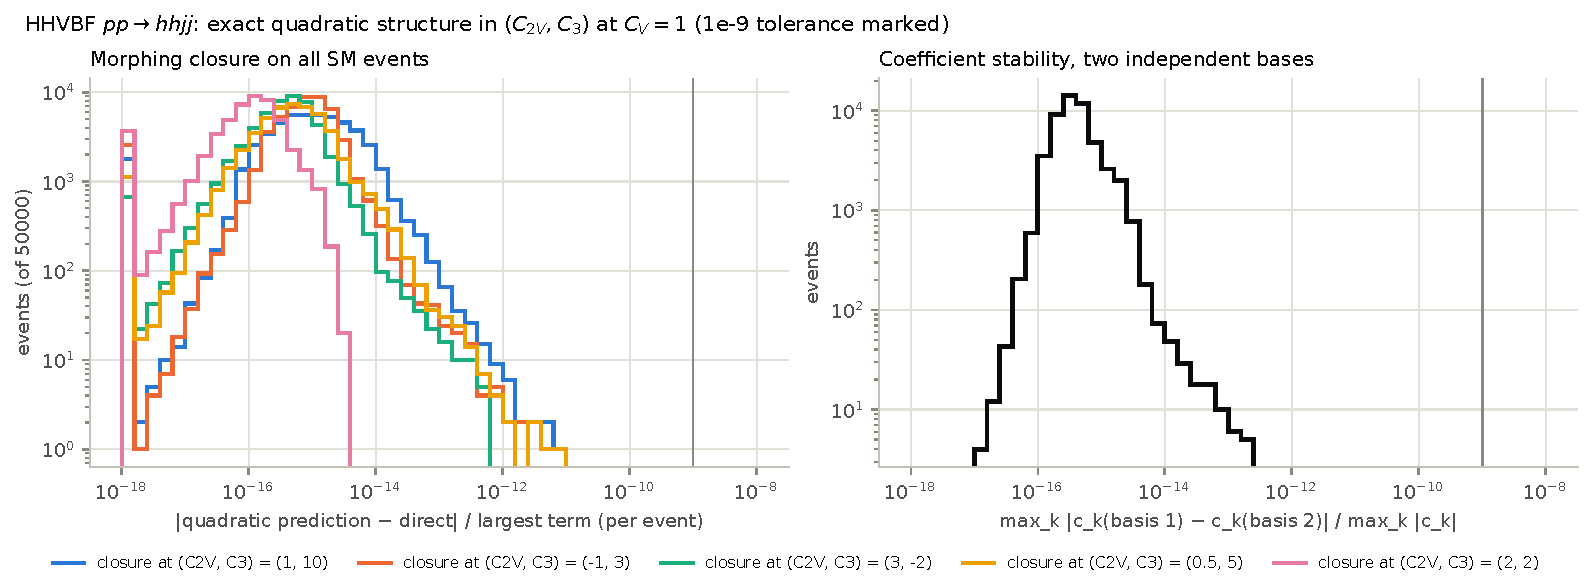
\includegraphics[width=0.75\textwidth]{study4_fig_4a.pdf}\caption{Study 4: difference between the quadratic morphing prediction and the direct evaluation of $|\M|^2$ at five coupling points, for all 50\,000 events.}\label{fig:s4a}\end{figure}
\begin{figure}[htbp]\centering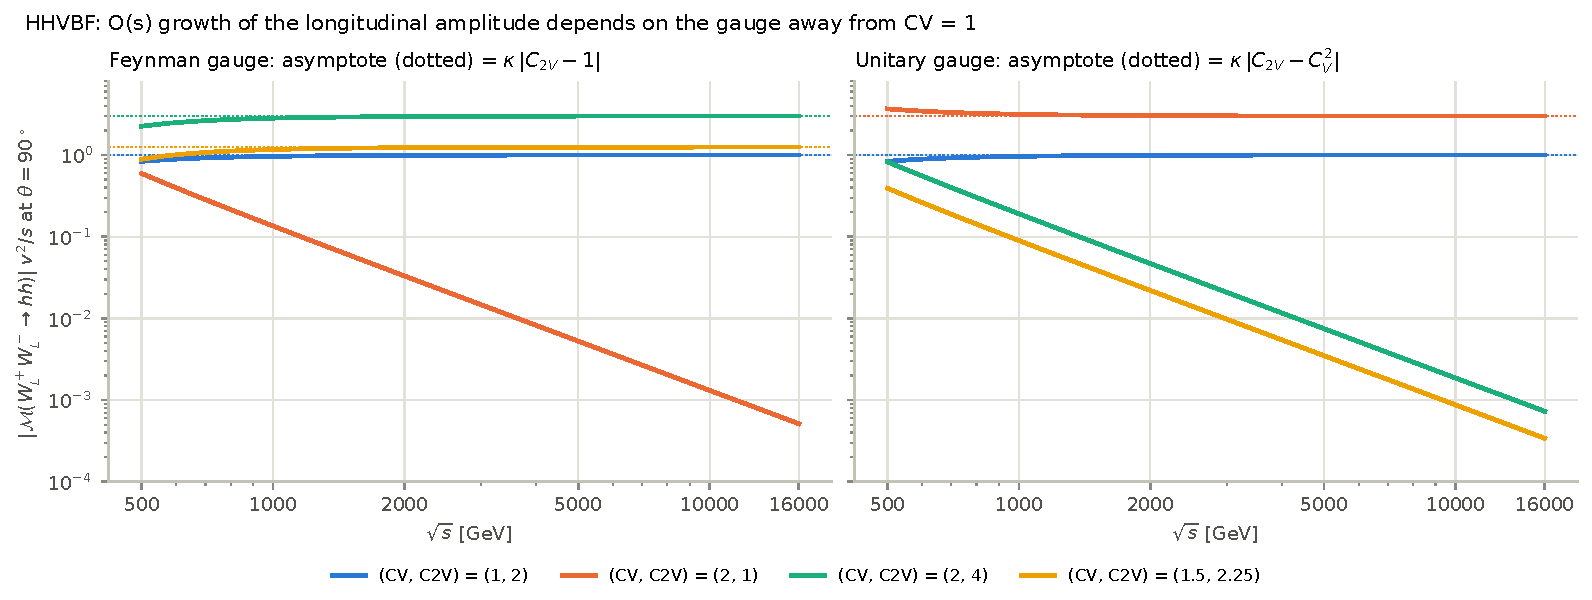
\includegraphics[width=0.8\textwidth]{study4_fig_4c.pdf}\caption{Study 4: energy growth of the longitudinal $W_LW_L\to hh$ amplitude in the HHVBF model, in Feynman and in unitary gauge, for four coupling choices.}\label{fig:s4c}\end{figure}

\subsection{Study 5: effective field theory operators}
\textbf{What is tested.} That Wilson coefficients behave as run-time parameters with the structure an effective field theory requires, and that the amplitude-level order window reproduces \mg.

\textbf{Figure~\ref{fig:s5a}.} For four operators of the Higgs sector of SMEFTsim~\cite{Brivio:2017btx,Brivio:2020onw} ($c_H$, $c_{H\Box}$, $c_{HDD}$, $c_{HW}$) the figure shows $|\M|^2$ for $u d\to u d h h$ at fixed kinematics versus the value of the coefficient, split into the Standard-Model part, the interference with the operator (linear in the coefficient) and the operator's own square (quadratic). With at most one insertion per amplitude (\code{set\_amp\_orders(\{"NP": (0, 1)\})}) the total is an exact parabola: fitted from three points it reproduces three others to $5\times10^{-15}$, and the linear piece equals the interference obtained directly from the single-insertion amplitude to $4\times10^{-16}$. The same window reproduces \mg's \code{NP<=1} to $3\times10^{-14}$, and without the window the full result reproduces \mg's \code{NP<=6}. With every insertion kept, the polynomial degree measured by \ufoamp{} is 2, 4, 8 and 4 for the four operators (reproducing $|\M|^2$ to $4\times10^{-15}$) --- which is why the window exists.

\textbf{Figure~\ref{fig:s5b}.} Two four-lepton operators of SMEFTsim, $c_{ll}$ and $c_{ll}'$, describe the same interaction with the fermion lines connected differently; a Fierz identity says they give equal amplitudes for $e^+e^-\to\mu^+\mu^-$. \ufoamp{} reproduces this to $7\times10^{-17}$ for all helicities over $-5\le c\le5$ --- a sharp test of its handling of four-fermion vertices and fermion signs. The figure also shows that, unless the input-scheme shifts of $c_{ll}'$ are frozen, the two differ by 11\% in amplitude, because $c_{ll}'$ enters the relation between $G_F$ and the gauge couplings: a subtlety of the model that \ufoamp{} reproduces rather than hides.
\begin{figure}[htbp]\centering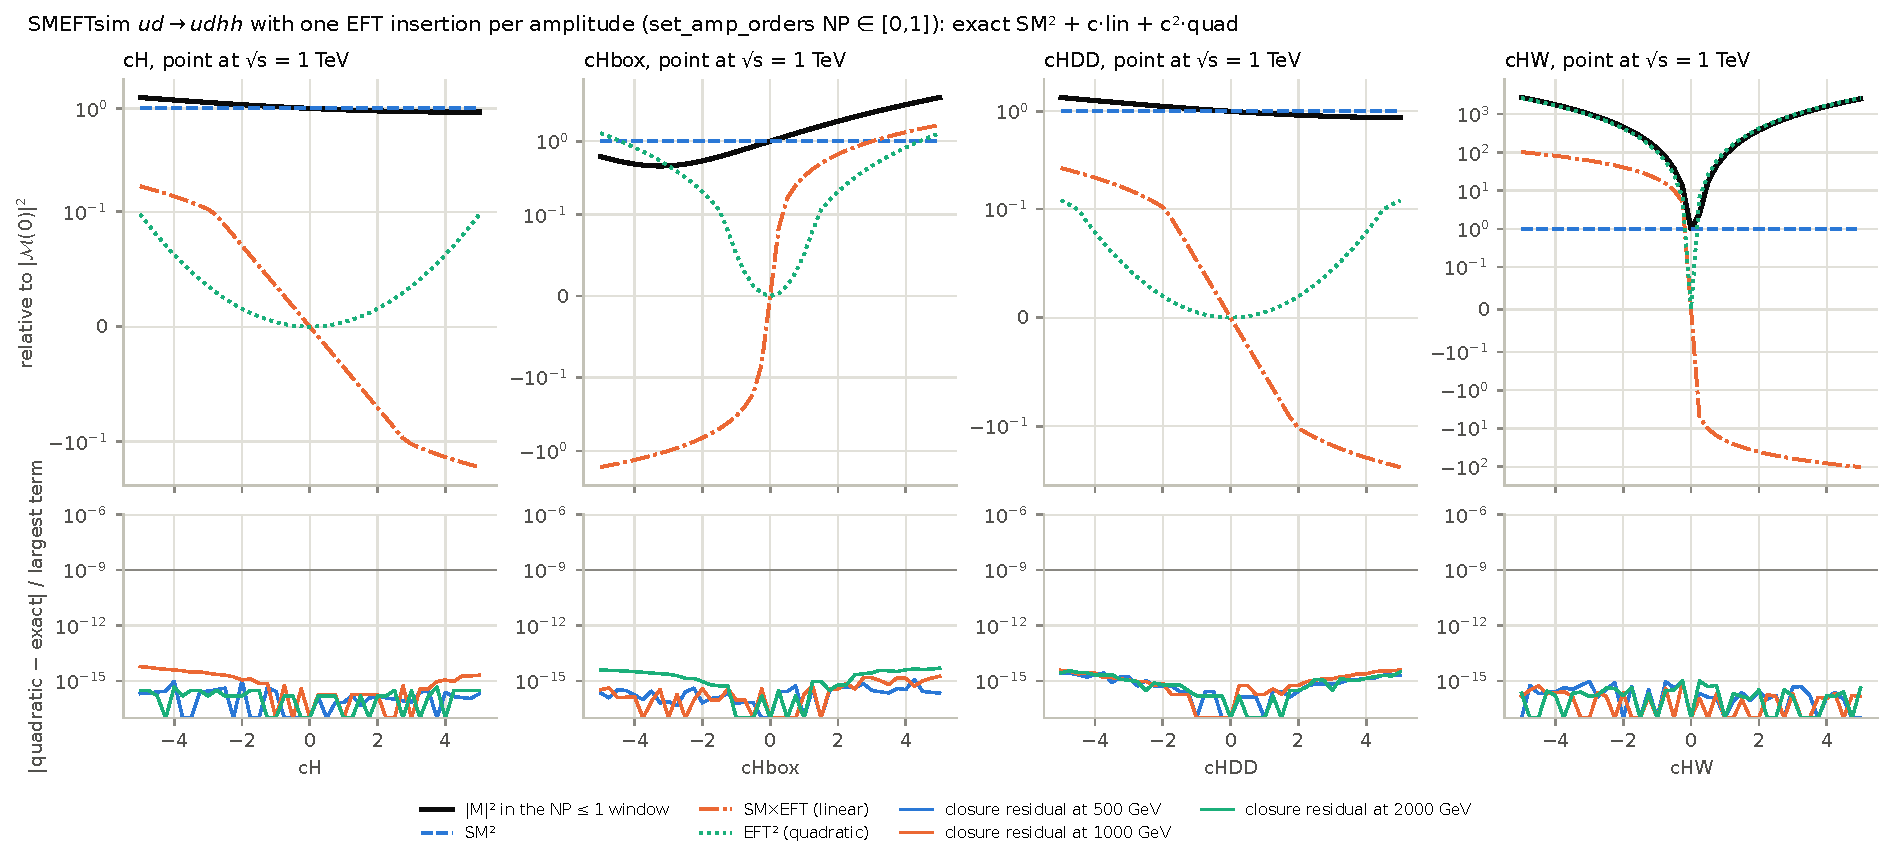
\includegraphics[width=0.9\textwidth]{study5_fig_5a.pdf}\caption{Study 5: $|\M|^2$ versus a Wilson coefficient with one insertion per amplitude, split into Standard Model, interference and operator-squared pieces.}\label{fig:s5a}\end{figure}
\begin{figure}[htbp]\centering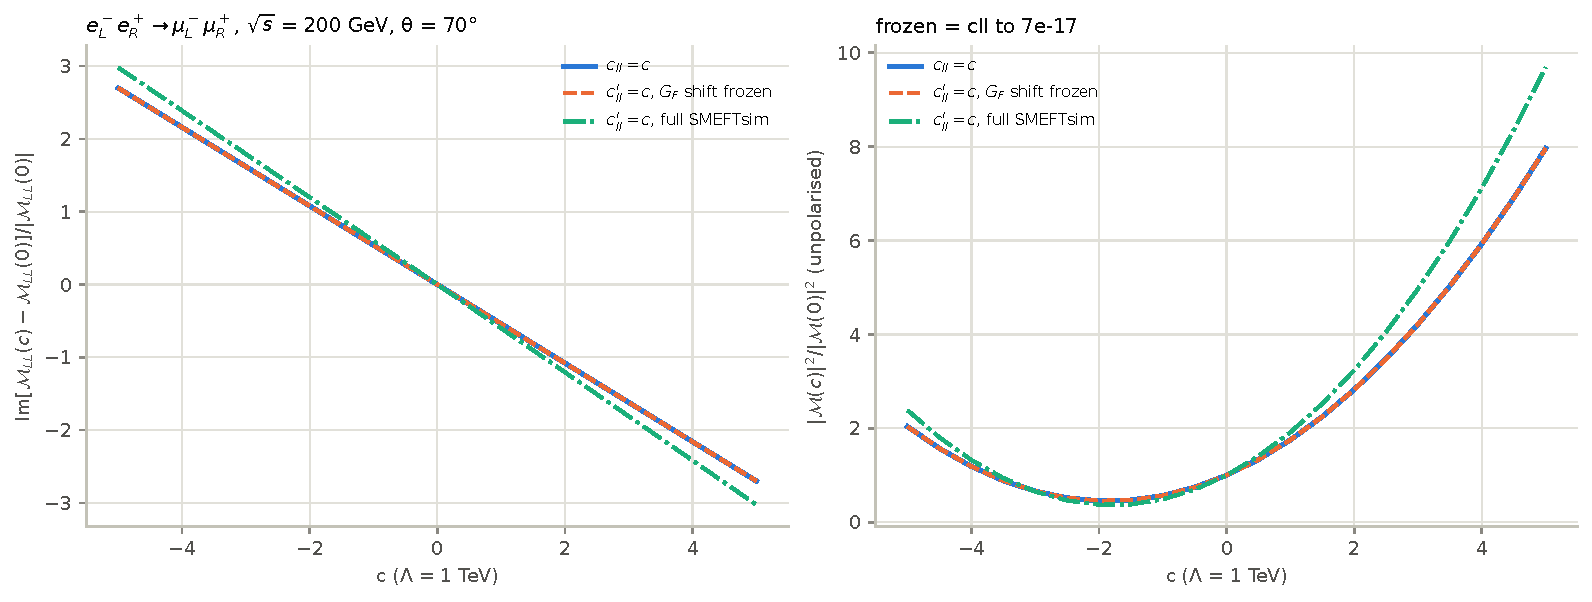
\includegraphics[width=0.8\textwidth]{study5_fig_5b.pdf}\caption{Study 5: the Fierz identity between the two four-lepton operators, and the effect of the input-scheme shift.}\label{fig:s5b}\end{figure}

\subsection{Study 6: derivatives with the JAX backend}
\textbf{What is tested.} That the compiled backend gives the same numbers as the NumPy one, that its automatically computed derivatives are exact, and what they are useful for.

\textbf{Numbers.} For $u d\to u d h h$ the JAX backend agrees with NumPy to $2\times10^{-14}$; its derivatives of $|\M|^2$ with respect to $C_{2V}$ and $C_3$ agree with the exact derivatives of the morphing polynomial of study~4 to $5\times10^{-14}$ (first derivatives) and $3\times10^{-14}$ (second derivatives), at 0.03\,ms per event for $|\M|^2$ and 0.04\,ms for the gradient, against 1.5\,ms and 9\,ms (six evaluations) with NumPy.

\textbf{Figure~\ref{fig:s6b}.} For $W^+W^-\to hh$ in SMEFTsim the derivative of $|\M|^2$ with respect to $c_{HW}$ and $c_{HDD}$ at the Standard-Model point --- the interference term --- is shown separately for the longitudinal, mixed and transverse helicity classes as a function of energy, together with the ratio of the operator's effect to the Standard Model. The derivatives agree with the interference computed directly to $5\times10^{-11}$. The plot reads off which operator affects which polarisation: $c_{HDD}$ acts on longitudinal $W$'s (its interference grows like $s$), $c_{HW}$ on transverse ones (its effect relative to the Standard Model grows like $s$ in the mixed class, where the Standard-Model amplitude falls like $1/s$).

\textbf{Figure~\ref{fig:s6c}.} On 5\,000 events of the $pp\to hhjj$ sample, the derivatives divided by $|\M|^2$ are the observables $O_{C_{2V}}=(\partial|\M|^2/\partial C_{2V})/|\M|^2$ and $O_{C_3}$ that are, by construction, the most sensitive to the two couplings; they agree with the derivatives of the stored morphing coefficients to $5\times10^{-13}$. Their distributions and their dependence on $m_{hh}$ show that at high mass the trilinear coupling decouples ($O_{C_3}\to0$) while $C_{2V}$ drives the behaviour.
\begin{figure}[htbp]\centering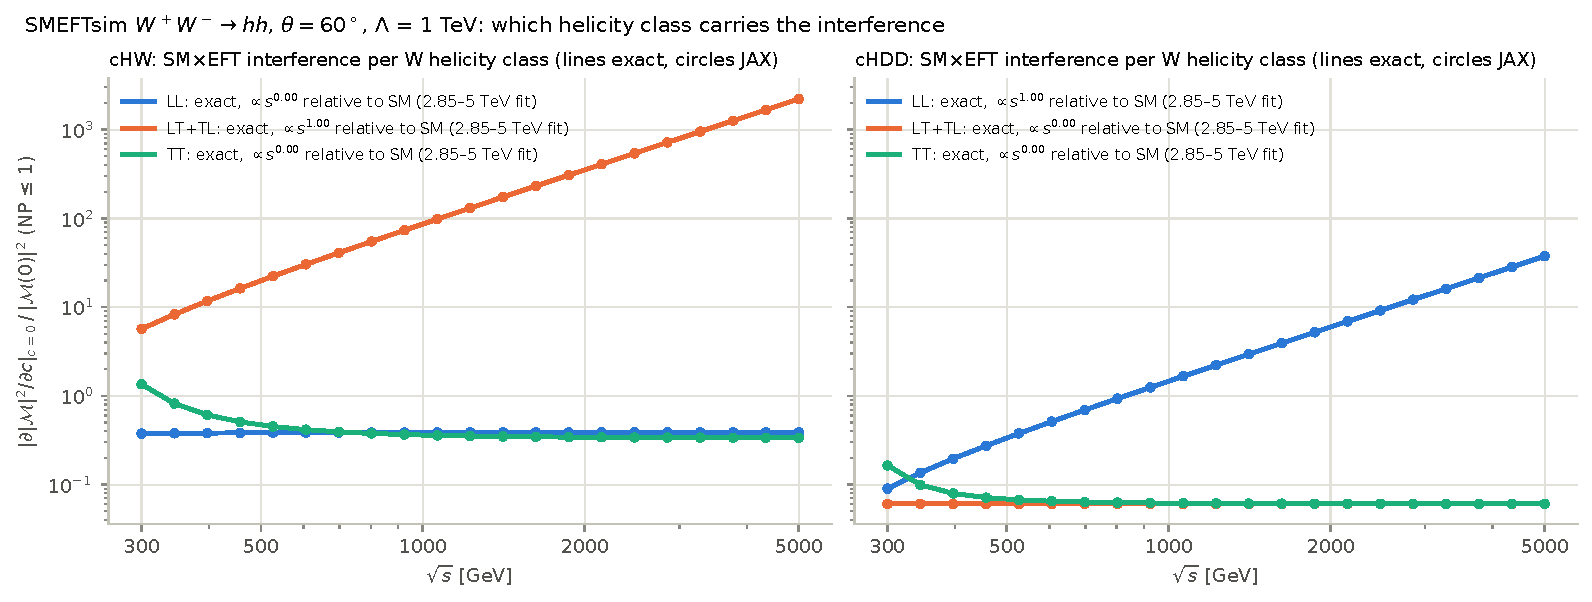
\includegraphics[width=0.9\textwidth]{study6_fig_6b.pdf}\caption{Study 6: per-helicity-class effect of two operators on $W^+W^-\to hh$ versus energy, and the derivative of $|\M|^2$ at the Standard-Model point from automatic differentiation.}\label{fig:s6b}\end{figure}
\begin{figure}[htbp]\centering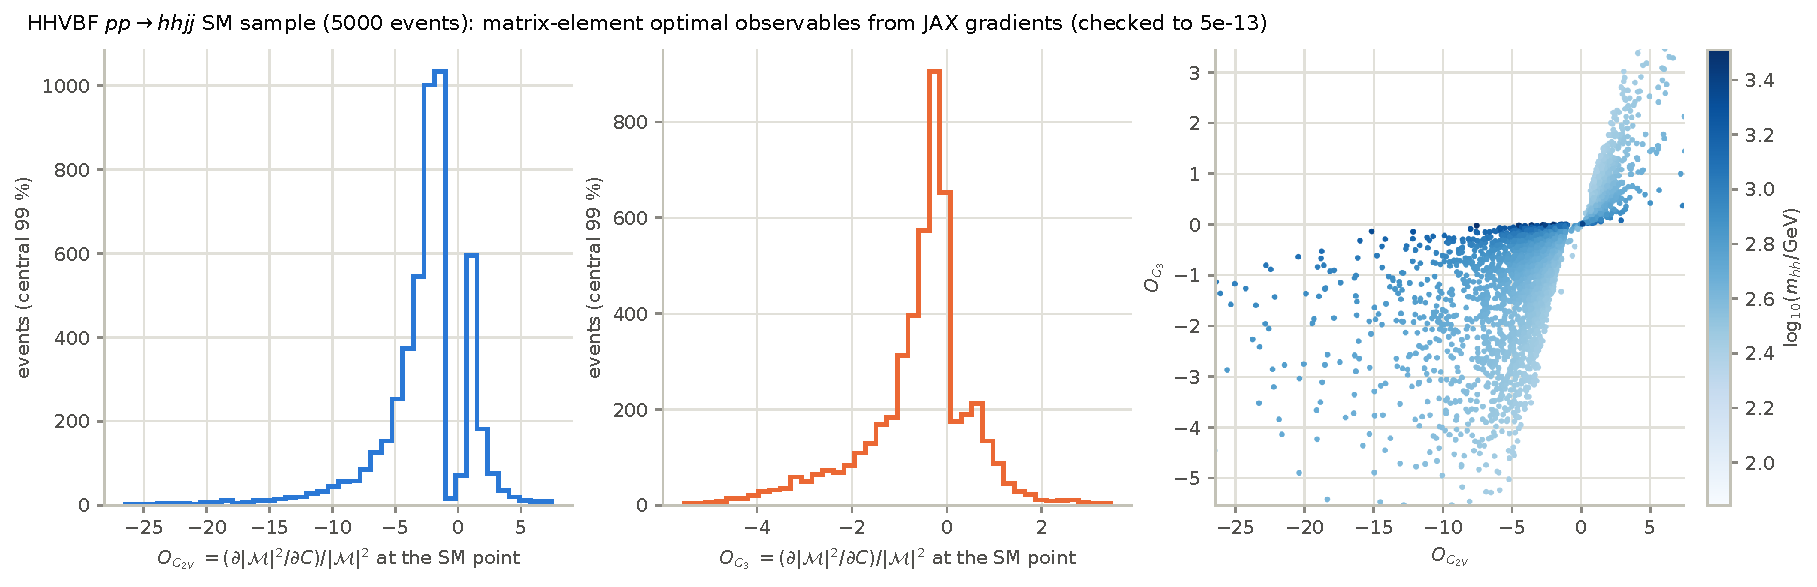
\includegraphics[width=0.9\textwidth]{study6_fig_6c.pdf}\caption{Study 6: matrix-element observables for $C_{2V}$ and $C_3$, computed from the derivatives of $|\M|^2$, on the $pp\to hhjj$ sample.}\label{fig:s6c}\end{figure}


\begin{thebibliography}{99}\small
\bibitem{Degrande:2011ua} C.~Degrande, C.~Duhr, B.~Fuks, D.~Grellscheid, O.~Mattelaer, T.~Reiter, \emph{UFO -- The Universal FeynRules Output}, Comput.\ Phys.\ Commun.\ 183 (2012) 1201, arXiv:1108.2040.
\bibitem{Darme:2023jdn} L.~Darm\'e et al., \emph{UFO 2.0: the `Universal Feynman Output' format}, Eur.\ Phys.\ J.\ C 83 (2023) 631, arXiv:2304.09883.
\bibitem{Alwall:2011uj} J.~Alwall, M.~Herquet, F.~Maltoni, O.~Mattelaer, T.~Stelzer, \emph{MadGraph 5: going beyond}, JHEP 06 (2011) 128, arXiv:1106.0522.
\bibitem{Alwall:2014hca} J.~Alwall et al., \emph{The automated computation of tree-level and next-to-leading order differential cross sections, and their matching to parton shower simulations}, JHEP 07 (2014) 079, arXiv:1405.0301.
\bibitem{deAquino:2011ub} P.~de~Aquino, W.~Link, F.~Maltoni, O.~Mattelaer, T.~Stelzer, \emph{ALOHA: Automatic Libraries Of Helicity Amplitudes for Feynman diagram computations}, Comput.\ Phys.\ Commun.\ 183 (2012) 2254, arXiv:1108.2041.
\bibitem{Murayama:1992gi} H.~Murayama, I.~Watanabe, K.~Hagiwara, \emph{HELAS: HELicity Amplitude Subroutines for Feynman diagram evaluations}, KEK-91-11 (1992).
\bibitem{Hagiwara:1985yu} K.~Hagiwara, D.~Zeppenfeld, \emph{Helicity amplitudes for heavy lepton production in $e^+e^-$ annihilation}, Nucl.\ Phys.\ B 274 (1986) 1.
\bibitem{Berends:1987me} F.~A.~Berends, W.~T.~Giele, \emph{Recursive calculations for processes with $n$ gluons}, Nucl.\ Phys.\ B 306 (1988) 759.
\bibitem{Kanaki:2000ey} A.~Kanaki, C.~G.~Papadopoulos, \emph{HELAC: a package to compute electroweak helicity amplitudes}, Comput.\ Phys.\ Commun.\ 132 (2000) 306, arXiv:hep-ph/0002082.
\bibitem{Moretti:2001zz} M.~Moretti, T.~Ohl, J.~Reuter, \emph{O'Mega: an optimizing matrix element generator}, arXiv:hep-ph/0102195.
\bibitem{Duhr:2006iq} C.~Duhr, S.~H\"oche, F.~Maltoni, \emph{Color-dressed recursive relations for multi-parton amplitudes}, JHEP 08 (2006) 062, arXiv:hep-ph/0607057.
\bibitem{Gleisberg:2008fv} T.~Gleisberg, S.~H\"oche, \emph{Comix, a new matrix element generator}, JHEP 12 (2008) 039, arXiv:0808.3674.
\bibitem{Hoche:2014kca} S.~H\"oche, S.~Kuttimalai, S.~Schumann, F.~Siegert, \emph{Beyond Standard Model calculations with Sherpa}, Eur.\ Phys.\ J.\ C 75 (2015) 135, arXiv:1412.6478.
\bibitem{Bothmann:2023gew} E.~Bothmann, T.~Childers, W.~Giele, S.~H\"oche, J.~Isaacson, M.~Knobbe, \emph{A portable parton-level event generator for the high-luminosity LHC}, SciPost Phys.\ 17 (2024) 081, arXiv:2311.06198.
\bibitem{Maltoni:2002mq} F.~Maltoni, K.~Paul, T.~Stelzer, S.~Willenbrock, \emph{Color-flow decomposition of QCD amplitudes}, Phys.\ Rev.\ D 67 (2003) 014026, arXiv:hep-ph/0209271.
\bibitem{Denner:1992vza} A.~Denner, H.~Eck, O.~Hahn, J.~K\"ublbeck, \emph{Feynman rules for fermion-number-violating interactions}, Nucl.\ Phys.\ B 387 (1992) 467.
\bibitem{Denner:1999gp} A.~Denner, S.~Dittmaier, M.~Roth, D.~Wackeroth, \emph{Predictions for all processes $e^+e^-\to 4$ fermions $+\gamma$}, Nucl.\ Phys.\ B 560 (1999) 33, arXiv:hep-ph/9904472.
\bibitem{Denner:2005fg} A.~Denner, S.~Dittmaier, M.~Roth, L.~H.~Wieders, \emph{Electroweak corrections to charged-current $e^+e^-\to4$ fermion processes: technical details and further results}, Nucl.\ Phys.\ B 724 (2005) 247, arXiv:hep-ph/0505042.
\bibitem{Baur:1995aa} U.~Baur, D.~Zeppenfeld, \emph{Finite-width effects and gauge invariance in radiative $W$ production and decay}, Phys.\ Rev.\ Lett.\ 75 (1995) 1002, arXiv:hep-ph/9503344.
\bibitem{Cornwall:1974km} J.~M.~Cornwall, D.~N.~Levin, G.~Tiktopoulos, \emph{Derivation of gauge invariance from high-energy unitarity bounds on the S matrix}, Phys.\ Rev.\ D 10 (1974) 1145.
\bibitem{Lee:1977eg} B.~W.~Lee, C.~Quigg, H.~B.~Thacker, \emph{Weak interactions at very high energies: the role of the Higgs-boson mass}, Phys.\ Rev.\ D 16 (1977) 1519.
\bibitem{Chanowitz:1985hj} M.~S.~Chanowitz, M.~K.~Gaillard, \emph{The TeV physics of strongly interacting W's and Z's}, Nucl.\ Phys.\ B 261 (1985) 379.
\bibitem{BuarqueFranzosi:2019boy} D.~Buarque~Franzosi, O.~Mattelaer, R.~Ruiz, S.~Shil, \emph{Automated predictions from polarized matrix elements}, JHEP 04 (2020) 082, arXiv:1912.01725.
\bibitem{Ballestrero:2017bxn} A.~Ballestrero, E.~Maina, G.~Pelliccioli, \emph{W boson polarization in vector boson scattering at the LHC}, JHEP 03 (2018) 170, arXiv:1710.09339.
\bibitem{Ballestrero:2019qoy} A.~Ballestrero, E.~Maina, G.~Pelliccioli, \emph{Polarized vector boson scattering in the fully leptonic WZ and ZZ channels at the LHC}, JHEP 09 (2019) 087, arXiv:1907.04722.
\bibitem{Denner:2020bcz} A.~Denner, G.~Pelliccioli, \emph{Polarized electroweak bosons in $W^+W^-$ production at the LHC including NLO QCD effects}, JHEP 09 (2020) 164, arXiv:2006.14867.
\bibitem{Artoisenet:2010cn} P.~Artoisenet, V.~Lema\^itre, F.~Maltoni, O.~Mattelaer, \emph{Automation of the matrix element reweighting method}, JHEP 12 (2010) 068, arXiv:1007.3300.
\bibitem{Mattelaer:2016gcx} O.~Mattelaer, \emph{On the maximal use of Monte Carlo samples: re-weighting events at NLO accuracy}, Eur.\ Phys.\ J.\ C 76 (2016) 674, arXiv:1607.00763.
\bibitem{ATL-PHYS-PUB-2015-047} ATLAS Collaboration, \emph{A morphing technique for signal modelling in a multidimensional space of coupling parameters}, ATL-PHYS-PUB-2015-047 (2015).
\bibitem{Brehmer:2019xox} J.~Brehmer, F.~Kling, I.~Espejo, K.~Cranmer, \emph{MadMiner: machine learning-based inference for particle physics}, Comput.\ Softw.\ Big Sci.\ 4 (2020) 3, arXiv:1907.10621.
\bibitem{Atwood:1991ka} D.~Atwood, A.~Soni, \emph{Analysis for magnetic moment and electric dipole moment form factors of the top quark via $e^+e^-\to t\bar t$}, Phys.\ Rev.\ D 45 (1992) 2405.
\bibitem{Diehl:1993br} M.~Diehl, O.~Nachtmann, \emph{Optimal observables for the measurement of three-gauge-boson couplings in $e^+e^-\to W^+W^-$}, Z.\ Phys.\ C 62 (1994) 397.
\bibitem{Brehmer:2016nyr} J.~Brehmer, K.~Cranmer, F.~Kling, T.~Plehn, \emph{Better Higgs boson measurements through information geometry}, Phys.\ Rev.\ D 95 (2017) 073002, arXiv:1612.05261.
\bibitem{Heinrich:2022xfa} L.~Heinrich, M.~Kagan, \emph{Differentiable matrix elements with MadJax}, J.\ Phys.\ Conf.\ Ser.\ 2438 (2023) 012137, arXiv:2203.00057.
\bibitem{Bradbury:2018jax} J.~Bradbury et al., \emph{JAX: composable transformations of Python+NumPy programs}, \url{http://github.com/google/jax} (2018).
\bibitem{Kleiss:1985gy} R.~Kleiss, W.~J.~Stirling, S.~D.~Ellis, \emph{A new Monte Carlo treatment of multiparticle phase space at high energies}, Comput.\ Phys.\ Commun.\ 40 (1986) 359.
\bibitem{Ellis:1996mzs} R.~K.~Ellis, W.~J.~Stirling, B.~R.~Webber, \emph{QCD and collider physics}, Cambridge University Press (1996).
\bibitem{Heinemeyer:2013tqa} LHC Higgs Cross Section Working Group, \emph{Handbook of LHC Higgs cross sections: 3. Higgs properties}, CERN-2013-004, arXiv:1307.1347.
\bibitem{Brivio:2017btx} I.~Brivio, Y.~Jiang, M.~Trott, \emph{The SMEFTsim package, theory and tools}, JHEP 12 (2017) 070, arXiv:1709.06492.
\bibitem{Brivio:2020onw} I.~Brivio, \emph{SMEFTsim 3.0 -- a practical guide}, JHEP 04 (2021) 073, arXiv:2012.11343.
\end{thebibliography}

\end{document}
